
\section{Introduction}
Imagine being a software development manager and hearing one of the worst possible pieces of news. One of your top engineers, Dakota, just gave notice and is moving on to a new opportunity. You might be torn with mixed emotions. On one hand, you are excited because the new position provides a great career opportunity for someone you respect. On the other hand, you might worry about your project. How is the team going to overcome this disruption? You have been investing in this engineer. Your investment and the engineer's entire accumulated knowledge about the code is walking out the door. As one of your top performers, Dakota worked on the most important aspects, the trickiest parts, of your system. How long is it going to take others to ramp up on the code that Dakota owned? How is this loss in productivity going to affect future development? 

Conventional wisdom says that team churn is detrimental to project success and that extensive documentation is needed to mitigate this effect. Unfortunately, documentation quickly becomes out-of-date and unreliable \cite{Lethbridge2003Documentation}, undermining this approach. During a grounded theory study, we observed projects succeed despite high disruption and little documentation. This raised the following research question: \quotes{How do the observed teams develop software effectively while overcoming team disruption?}

Exploring this question resulted in a descriptive theory of \quotes{Sustainable Software Development.} The theory explains how a collection of synergistic principles, policies, and practices help develop software effectively while overcoming team disruption. This is done by engendering a positive attitudes towards team disruption, encouraging knowledge sharing and continuity, as well as caring about high code quality. Here, \textit{team disruption} refers to substantial ongoing changes in team composition, like team members joining or leaving, as well as temporary vacations or leave of absence. 

In Section \ref{RelatedWork}, we present related work on Extreme Programming and team disruption. In Section \ref{ResearchMethod}, we review how we employed Constructivist Grounded Theory to derive a descriptive theory supported by empirical data. We also present the research context, introducing both the company and one of the five projects under study. In Section \ref{Theory}, we describe the theory and how its principles, policies, and practices work together to achieve software development sustainability. In Section \ref{TheoryEvaluation}, we evaluate the theory using established criteria for evaluating a grounded theory. In the last sections, we examine threats to research validity, consider future research, and conclude the research.
\section{Related Work}
\label{RelatedWork}
In Extreme Programming \cite{BeckExtremeProgramming2004}, Kent Beck describes a set of interdependent practices that manage feature development (much like Scrum \cite{SchwaberScrum}), as well as technical practices that facilitate a collaborative team environment. Extreme Programming comprises 13 primary practices and 11 corollary practices. 

One Extreme Programming practice, collective ownership, simply means that \quotes{anyone on the team can improve any part of the system at any time.} Beck contrasts collective ownership with \quotes{no ownership} and \quotes{individual ownership.} With collective ownership, every developer takes responsibility for the whole of the system. When developers see opportunities to improve the code, they go ahead and improve it if it makes their life easier \cite{BeckExtremeProgramming2000}. Later, \quotes{collective ownership} was renamed to \quotes{shared code} \cite{BeckExtremeProgramming2004}. 

One Extreme Programming practice contributing to collective code ownership is pair programming. Pair programming is where production code is created by two developers working together at a single computer \cite{BeckExtremeProgramming2004}. Extreme Programming does not prescribe how pairs are formed, or for how long a pair works together.  However, Extreme Programming recommends rotating pairs frequently by switching at natural breaks in development. Williams presents a pair rotation strategy for maintaining specialization, by \quotes{choosing the right partner for the right situation}  \cite{Williams2002}. People are assigned modules of the code to own based upon expertise and find partners from neighboring modules. While knowledge is shared with pairing, one person owns every story that touches that part of the system, building individual code ownership. In one case study, the project started with a pair rotation strategy based on skillsets but evolved into a daily rotation determined randomly \cite{Vanhanen2007}. Some teams use a pair programing matrix \cite{AlaverdyanPairProgrammingMatrix} (also called a pairing ladder \cite{Davies2009AgileCoaching}) to track who has paired with whom for the purpose of pairing people who have not paired recently.

Truck Number is \quotes{The size of the smallest set of people in a project such that, if all of them got hit by a truck, the project would be in trouble.} \cite{WikiTruckNumber}. Truck Number, or Bus Count, reminds management about the effects of disruptive events for a team. In 1994, Coplien \cite{Coplien1994} mentions \quotes{Truck Number} as a risk to his Solo Virtuoso pattern of using only one talented developer to create a software system. Awati suggests that Truck Number can be increased by reducing complexity, cross-training, and documentation \cite{AwatiBusFactor}, all of which are found in Extreme Programming. However, Extreme Programming implements \quotes{documentation} as discoverable, intention revealing code. Ricca \cite{Ricca2011TruckFactor} examines the difficulty in computing the Truck Number. 

Rigby quantifies turnover using knowledge at risk analysis on abandoned files  \cite{Rigby2016Turnover}. A line of code is abandoned if the most recent contributor has left the company.  A file is abandoned if more than 90\% of the lines in the file are abandoned.  Izquierdo examines how teams managed orphaned code \cite{Izquierdo2009Turnover}. Joseph examines job turnovers to understand the reasons developers leave their company  \cite{Joseph2007Turnover}.  
\section{Research Method}
\label{ResearchMethod}
\subsection{Constructivist Grounded Theory}

We adopted Grounded Theory \cite{Charmaz}, which provides an iterative approach to data collection, data coding, and analysis resulting in an emergent theory. We selected Charmaz' Constructivist approach to Grounded Theory, which \quotes{emphasizes understanding and acknowledges that data, interpretations, and resulting theory depend on the researcher's view} \cite{StolGTinSE}. The two primary data sources were field notes collected during continuous participant observations of a seven-month project and interviews with Pivotal software engineers, interaction designers, and product managers. Interviews were recorded, transcribed, coded, and analyzed using constant comparison. In addition, the primary researcher was involved in four other projects as participant-observer.

Grounded Theory immerses the researcher within the context of the research subject from the point of view of the participants. As the research progresses, Grounded Theory allows the researcher to \quotes{incrementally direct the data collection and theoretical ideas.} The theory provides a starting place for inquiry, not a specific goal known at the beginning of the research. As we interact with the data, the data influence how we progress and alter the research direction. When starting a grounded theory research study, the core question is, \quotes{What is happening here?} \cite{GlaserTheoreticalSensitivity}. Our initial core question was \quotes{What is happening at Pivotal when it comes to software development?}
\subsection{Participants}
The first author interviewed 21 interaction designers, product managers, and software engineers who had experience with Pivotal's software development process. They were distributed across four different Pivotal offices. Interaction designers identify user needs predominately through user interviews; create and validate user experience with mockups; determine the visual design of a product; and support engineering during implementation. Product managers are responsible for identifying and prioritizing features, converting features into stories, prioritizing stories in a backlog, and communicating the stories to the engineers. Software engineers implement the solution. Participants were not paid for their time. 
\subsection{Data Collection}
The primary researcher relied on \quotes{intensive interviews,} which are \quotes{open-ended yet directed, shaped yet emergent, and paced yet unrestricted} \cite{Charmaz}. Open-ended questions were used to enter into the participant's personal perspective within the context of the research question. The interviewer attempts to abandon assumptions to better understand and explore the interviewee's perspective. Charmaz \cite{Charmaz} contrasts intensive interviews from informational interviews, which facilitate collecting accurate `facts' and investigative interviews that attempt to reveal hidden intentions or expose practices and policies. 
 
The initial interviews were open-ended explorations starting with the question, \quotes{Please draw on this sheet of paper your view of Pivotal's software development process.} The interviewer specifically did not force initial topics and merely followed the path of the interviewee. 

While exploring new emergent core categories, whenever possible, the researcher initiated subsequent interviews with open-ended questions.  For example, asking the participant, \quotes{Please draw your feelings about the code} often resulted in conversations about code ownership. 

Each interview was transcribed into a Word document with timecode stamps for each segment.

In addition to collecting data from interviews, the primary researcher collected field notes while working as an engineer on the project described in Section \ref{ProjectQuattuor}. The field notes comprised multiple paragraph entries recorded several times a week, collected over a seven month period. These notes described individual and collective actions, captured what participants defined as interesting or problematic, and included anecdotes and observations. 
\subsection{Data Analysis}
Data analysis began with line-by-line coding as recommended by Charmaz \cite{Charmaz}. Coding line-by-line helps the researcher identify nuanced interactions in the data and avoid jumping to conclusions. The data then advanced from these initial codes to focused codes, focused codes to core categories, and core categories to an emergent theory. 

After the initial coding, another researcher reviewed the initial codes while reading the transcripts and listening to the audio recording. We discussed the coding during weekly research collaboration meetings. To avoid missing insights from these discussions \cite{GlaserTheoreticalSensitivity}, we recorded and transcribed them into grounded theory memos. 
As data was collected and coded, initial codes were recorded in a spreadsheet and constant comparison was used to generate focused codes. Only ideas expressed by multiple interviewees informed focused codes and subsequent analysis. 
The researcher constantly compared new codes to existing codes to refine codes and eventually generate categories. The primary researcher periodically audited each category for cohesion by comparing its codes. When this became complex, the codes were printed on index cards, and then arranged and re-arranged until cohesive categories emerged. The researcher captured the analysis of codes, examinations of theoretical plausibility, and insights in memos. 
Constant comparison allowed the researcher to identify \quotes{the conceptual relationship between categories and their properties as they emerged} \cite{GlaserBasics}, leading to a resulting descriptive theory. The resulting theory is presented in Section \ref{Theory} and illustrated in Table \ref{SustainableSoftwareDevelopmentTable}. The table includes the main categories and their organization into principles, policies, and practices. Examples of quotes leading to some categories are presented in Table \ref{ChainOfEvidenceTable}.


\begin{table}[t]
\renewcommand{\arraystretch}{1.5}
\centering
\caption{Quotes for Selected Categories}
\label{ChainOfEvidenceTable}
\begin{tabular}{|p{3.15in}|}
\hline
Engendering Positive Attitudes Toward Team Disruption \\
\hline
\participantQuote{I'm excited when a new person joins the team. That person has experience that might add something to the project.} \\

\participantQuote{I like that people bring new energy. Projects often get into the state of a lull with the same people working on it and have the same cadence. New people bring a new perspective. [Two engineers recently joined] and it was really cool to see their fresh perspective. I always like people joining a project.} \\

\participantQuote{Team members go out of their way to make new teammates feel welcome and help ramp them up.} \\

\hline
Team Code Ownership \\
\hline
\participantQuote{I feel ownership of the code as a whole, and I feel empowered and able to go and work on any part of the codebase.} \\
\participantQuote{I don't feel like I have [individual] ownership. It's really a collaborative effort to achieve where we are today \ldots I feel like everybody owns this product.} \\
\participantQuote{There is a lot of emphasis that you are not your code.} \\
\participantQuote{I never feel like a specific piece is mine or something belongs to other people.}\\

\hline
Overlapping Pair Rotation \\
\hline
\participantQuote{To make sure that knowledge silos don't form we rotate pairs. As people work on specific stories and specific parts of the code, we want to share that knowledge.} \\

\participantQuote{Rotating pairs reduces knowledge silos and reduces the bus factor. We do not want the departure of one developer from the project to cripple the project.} \\

\participantQuote{We rotate pairs because everyone has a different set of knowledge. When you work with someone you get a little bit of that knowledge. The more you pair with them, the more knowledge you get.} \\

\hline
\end{tabular}
\end{table}


\subsection{Research Context}
\label{ResearchContext}

Pivotal is a large American software company (with 16 offices around the world), which provides solutions for cloud-based computing, big data, and agile development. 

This study focuses on one Pivotal subsidiary, Pivotal Labs, which provides agile developers, product managers, and interaction designers to other firms. Its mission is to deliver highly-crafted software products and provide a transformative experience for clients' engineering cultures. To change the client's development process, Pivotal combines the client's software engineers with Pivotal's engineers at a Pivotal office where they can experience Extreme Programming in an environment conducive to agile development. For startups, Pivotal engineers might be the first to work on the project. For enterprise clients, Pivotal provides additional engineering resources to accomplish new business goals. 

Pair programing ability is a strong pre-requisite for becoming a Pivotal Labs developer. During job interviews, applicants engage in multiple pair-programming rounds to reveal the applicant's ability to listen to and empathize with pairs. 

Typical teams include six developers, one interaction designer, and a product manager. The largest project in the history of the Palo Alto office had 28 developers while the smallest had 2. Larger projects are organized into smaller coordinating teams with one product manager per team and one or two interaction designers per team. 

Commonly utilized technologies include Angular, Android, backbone, iOS, Java, Rails, React, and Spring and are often deployed onto Pivotal's Cloud Foundry. 

Pivotal Labs has followed Extreme Programming \cite{BeckExtremeProgramming2004} since the late 1990's. While each team autonomously decides what is best for each project, the company culture strongly suggests following all of the core practices of Extreme Programming, including pair programming, test-driven development, weekly retrospectives, daily stand-ups, a prioritized backlog, and team code ownership, as well as Kanban's notion of work flowing through people.

We only observed teams in Pivotal Labs. Other teams, especially teams in other divisions, might have a different culture and follow different software practices.
\subsection{Project Context: Project Quattuor}
\label{ProjectQuattuor}
While we observed five projects in total, this paper focuses on Project Quattuor. This project shares many similarities with the other four. To preserve client confidentiality, we cannot reveal the exact nature of Project Quattuor; however, its purpose was to develop a mobile application for controlling expensive equipment.

The project lasted 43 weeks. The initial four weeks were called Discovery and Framing, where: 1) interaction designers investigate user needs through user interviews, 2) product managers define the features for the initial release based on those needs, 3) interaction designers create an initial interaction design and validate their mock-ups with users, and 4) engineers mitigate technology risks. Discovery and Framing was followed by code implementation, resulting in two releases to both the Apple store and Google play store.

\begin{figure}[t]
\centering
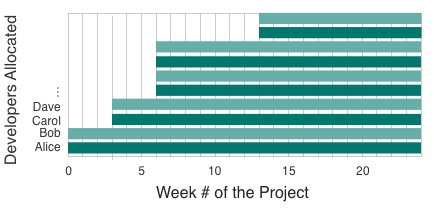
\includegraphics[width=\oneColumnWidth{}]{sustainable_software_development_images/OriginalDeveloperStaffingV3.jpg}
\caption{Planned Developer Staffing}
\label{PlannedDeveloperStaffing}
\end{figure}

The 35-person project consisted of an iOS team of 10 engineers, an android team of 10 engineers, and a Java back-end team of 8 engineers with the support of 2 to 4 interaction designers and 3 product managers. Here we focus on the iOS team. The first iOS release to the Apple store occurred in week 23. Given the success of the project, the client extended the engagement for a second iOS release that happened on week 43. 

Figure \ref{PlannedDeveloperStaffing} shows the staffing plan at the start of Project Quattuor. The plan was to start the project with two developers, while adding more developers as more tracks of work become available. Figure \ref{DeveloperStaffing} shows the actual staffing, which is quite different from the plan.

The bar chart on the top of Figure \ref{DeveloperStaffing}  shows when individual developers started and stopped working on the project, that there were five developers who were on the project for most of its duration, that 22 people actually worked on the project, and that the maximum team size was 12 developers working together at the same time. The graph on the bottom of Figure \ref{DeveloperStaffing} shows the total number of developers allocated to the project at any given week. Developers ramped up from week 5 to week 12, with an average of team size of 10 and a maximum of 12 developers.

Developers were routinely rotated and were replaced for various reasons, including promotions, medical leave, leaving the company, transferring to a different office, and vacations. Most importantly, the client was more concerned with feature development than cost, so absent developers were replaced, leading to 22 different people working on the same ten-person project. 

The ongoing rotation of team members likely undermined the team's sense of identity \cite{TuckmanModel}. In addition, the project experienced many challenges, including not having access to production back-end systems or expensive dependent physical components, and cultural differences between Pivotal and the client's deployment organization. Yet the team successfully completed the project. The client was delighted, even claiming that the team had delivered a multi-year project in 5 months by delivering the first release. 

Contrary to conventional wisdom, high team disruption did not appear to negatively influence the success of Project Quattuor. This observation raises our research question: \quotes{How do the observed teams develop software effectively while overcoming team disruption?}


%\begin{figure*}[t]
%\centering
%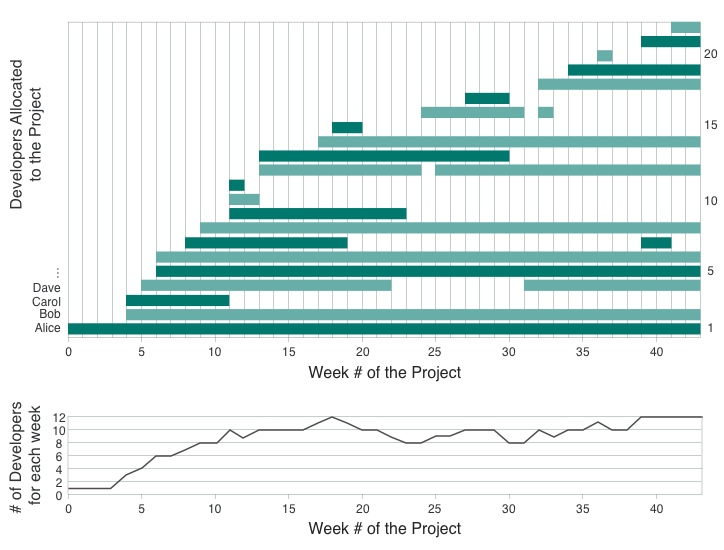
\includegraphics[width=\twoColumnWidth{}]{DeveloperStaffingV4.jpg}
%\caption{Actual Developer Staffing}
%\label{DeveloperStaffing}
%\end{figure*}

\begin{figure}[t]
\centering
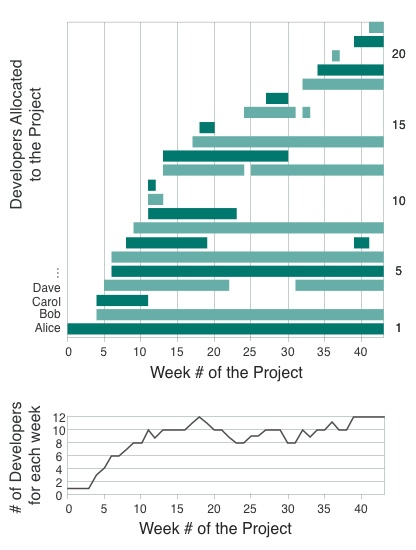
\includegraphics[width=\oneColumnWidth{}]{sustainable_software_development_images/DeveloperStaffingV7.jpg}
\caption{Actual Developer Staffing}
\label{DeveloperStaffing}
\end{figure}

\begin{table*}[t]
\renewcommand{\arraystretch}{1.5}
\centering
\caption{Theory of Sustainable Software Development: Principles, Policies, and Practices}
\label{SustainableSoftwareDevelopmentTable}
\begin{tabular}{|p{1.75in}|p{1.30in}|p{1.75in}|p{1.6in}|}
\hline
\multicolumn{4}{|c|}{Sustainable Software Development} \\
\hline
Underlying Principles & Policies & Removing Knowledge Silos Practices & Caretaking the Code Practices \\
\hline
Engendering Positive Attitudes Toward Team Disruption & Team Code Ownership & Continuous Pair Programming & TDD / BDD \\
Encouraging Knowledge Sharing and Continuity & Shared Schedule & Overlapping Pair Rotation & Continuous Refactoring \\
Caring about Code Quality & Avoid Technical Debt & Knowledge Pollination & Supported by Live on Master \\ 
\hline
\end{tabular}
\end{table*}


\section{Theory of Sustainable Software Development}
\label{Theory}

Sustainable software development refers to the ability and propensity of a software development team to mitigate the negative effects of major disruptions, especially team churn, on its productivity and effectiveness. Our theory of Sustainable Software Development, summarized in Table \ref{SustainableSoftwareDevelopmentTable}, is targeted towards software developers and has emerged from the grounded theory research described above. We hypothesize that sustainability emerges from synergistic principles, policies, and practices, which collectively explain how the observed Pivotal teams overcome disruption. The ability of any pair to work on any story while caring about the code is the primary mechanism by which these principles, policies, and practices mitigate disruption. 

In this section, we document each principle, policy, and practice.  For each policy and practice, we present how it is used at Pivotal, and discuss anti-patterns and potential alternatives. We provide deeper descriptions for practices rarely documented in the literature.
\subsection{Principles}

\subsubsection{Engendering Positive Attitudes Toward Disruption}
Conventional wisdom says that team disruption should be avoided. Yet, team disruption is a reality in the industry, as exemplified by Project Quattuor where only five of twenty-two developers worked on the project for most of its duration (see Figure \ref{DeveloperStaffing}). However, the observed organization engendered a positive attitude towards disruption, transforming a challenge into an opportunity and hence demonstrating remarkable business agility. Team members rolling off the project were replaced as needed. New members rolling onto the project were viewed as an opportunity to improve the current code base by providing a fresh, new perspective. When a new team member did not understand the code base, he or she revealed issues with code discoverability. New team members often questioned the team's assumptions and challenged \quotes{cargo culting.} 

The first underlying principle of Sustainable Software Development is engendering an open and positive attitudes towards team disruption, transforming a challenge into an opportunity to improve code quality.

\subsubsection{Encouraging Knowledge Sharing and Continuity}
Despite the fresh perspectives added by new team members, team disruption could potentially result in significant knowledge loss for the organization. A set of policies and practices aiming at encouraging knowledge sharing and continuity mitigates this risk. These policies are Team Code Ownership, and Shared Schedule, while the practices are Continuous Pair Programming, Overlapping Pair Rotation, and Knowledge Pollination. (Refer to the following sections for more on these policies and practices.)

The second underlying principle of Sustainable Software Development is encouraging knowledge sharing and continuity, enabling the knowledge to spread from one developer to the next, and eventually reach the entire team. Knowledge sharing and continuity make the team more resistant to disruption. 

\subsubsection{Caring about Code Quality}

Enabling knowledge sharing and continuity does not guarantee sustainable development if the team starts incurring technical debt \cite{McConnellTechnicalDebt}. A set of policy and practices aimed at taking good care of the code itself mitigates this risk. The policy is Avoid Technical Debt, while the practices are Test-Driven Development / Behavior-Driven Development and Continuous Refactoring. (Refer to the following sections for more on these policy and practices.)

The third underlying principle of Sustainable Software Development is caring about code quality, hence avoiding technical debt and enabling sustainable team productivity.
\subsection{Policies}

\subsubsection{Team Code Ownership}

\textbf{Description:} Team code ownership conveys that any team member can modify any part of the team's code at any time. 

\textbf{Purpose:} Everyone on the team is responsible for the team's code. Simply saying \quotes{Any team member can modify any piece of the code} is not sufficient to achieve the desired result of team code ownership. We documented five factors that affect the team's sense of code ownership and eight risks observed on Pivotal teams \cite{SedanoTeamCodeOwnership}. Achieving team code ownership requires a set of enabling practices. These enabling practices aim at removing knowledge silos and taking good care of the code, as described in the following sections.

\textbf{At Pivotal:} Every developer is empowered to work on any part of the team's code and is encouraged to refactor any code section to improve its quality as needed, especially when code discoverability and readability is an issue.

\textbf{Anti-pattern:} Removing team code ownership makes sustainable software development challenging. Every line of code written via strong ownership creates a knowledge silo. Code reviews are a mitigation strategy with an asynchronous delay. When the delay is too long, merging code onto the master becomes problematic, which then places pressure to avoid Continuous Refactoring. 

\subsubsection{Shared Schedule}
\textbf{Description:} Shared Schedule signifies that all team members share the same work schedule. 

\textbf{Purpose:} Shared Schedule enables Continuous Pair Programming, Overlapping Pair Rotation, and Knowledge Pollination practices. With Shared Schedule, teams form new pairs at the beginning of the day. The evening becomes a natural interruption to the continuous software development workflow. 

\textbf{At Pivotal:} Team members at the Palo Alto office start working at 9:00 in the morning and leave at 6:00 in the evening, five days a week. This is done without management coercion; each team member agreed to this fixed schedule to achieve the benefits of Sustainable Software Development. When Shared Schedule is the normative, flexibility is possible for exceptions. For instance, seeing the doctor during the day is fine since it is important to take care of oneself.

Pivotal prefers for all team members to be co-located as it promotes synchronous and osmotic communication. As an exception, Project Quattuor was a two-office project with half the team members in Palo Alto and half the team members in San Francisco. Each day, developers in one location remotely paired with developers in the other location to spread the knowledge across the two offices. Future research could explore whether Sustained Software Development works for a distributed team with a Shared Schedule.

\textbf{Anti-pattern:} Flexible work hours potentially jeopardizes Continuous Pair Programming, Overlapping Pair Rotation, and Knowledge Pollination practices. A team with flexible work hours might find it difficult to pair program on all stories (as described in the Continuous Pair Programming practice). A team member consistently soloing from 8:00 am to 10:00 am might be building knowledge silos. 

When developers arrive whenever they feel like it, rotating pairs (as described under the Overlapping Pair Rotation practice) becomes awkward, as there is no longer a natural time to rotate pairs. Trying to schedule a time midday to rotate pairs feels artificial. Even if the team says they will rotate later in the day, once pairs get into their stories and form context on what needs to be done, they typically forget about re-pairing until it is time to go home.

Pivotal experimented with pairing when developers arrived, but this meant that developers coming early were making decisions for the team members who arrived later, hence loosing some benefits of pair programming. 

\textbf{Alternatives:} A possible mitigation strategy could be to adopt core work hours. Individuals would solo on simple cleanup chores outside of core hours, and switch to pair programming for feature development when the whole team is in the office. 

\subsubsection{Avoid Technical Debt}
\textbf{Description:} Technical Debt refers to delaying needed technical work, by taking technical shortcuts, usually in pursuit of calendar-driven software schedules \cite{McConnellTechnicalDebt}. 

\textbf{Purpose:} Avoid Technical Debt enables a team to balance feature development with Continuous Refactoring (as described under the Continuous Refactoring practice). When a team is pressured to finish work by a deadline, they might be tempted to focus on feature delivery, take on technical debt, and stop refactoring. When a team delays refactoring and takes on technical debt, the code becomes harder to work with, which in turn makes it more difficult for developers to rotate onto that part of the code base. There is a dialectic tension \cite{RalphProcessTheories} between Continuous Refactoring and delivering more features while accruing technical debt.

\textbf{At Pivotal:} A pair tends to create well-crafted code by avoiding shortcuts and short-term fixes. The team codes for the \quotes{present} by building the simplest solution for the current story. The team eschews over-engineering for potential future features. The team avoids technical debt by building the best solution for the moment at hand. When inheriting a large code base with existing technical debt, we observed a team actively paying down technical debt while delivering new features. 

\textbf{Anti-pattern:} On Project Quattuor, the product manager suggested that the team deliver more stories at the cost of technical debt to make a release date. Some team members followed this suggestion, skipped the refactoring step, and introduced harder to maintain code. This decision made it difficult for pairs to rotate onto parts of the code. Pairs making the decision to skip refactoring caused future pain for the next pair to work with that part of the code. Immediately after the first release, the team spent several weeks refactoring the code to pay down the debt and consistently deliver new features again. During stressful times it is critical for the team to double down on its practices and be more disciplined.
\subsection{Removing Knowledge Silos Practices}
This section presents practices for encouraging knowledge sharing and continuity, enabling the knowledge to spread from one developer to the next, and eventually reach the entire team, as illustrated in Figure 3, where letters A to F represent 6 developers working in pairs.

\begin{figure}[t]
\centering
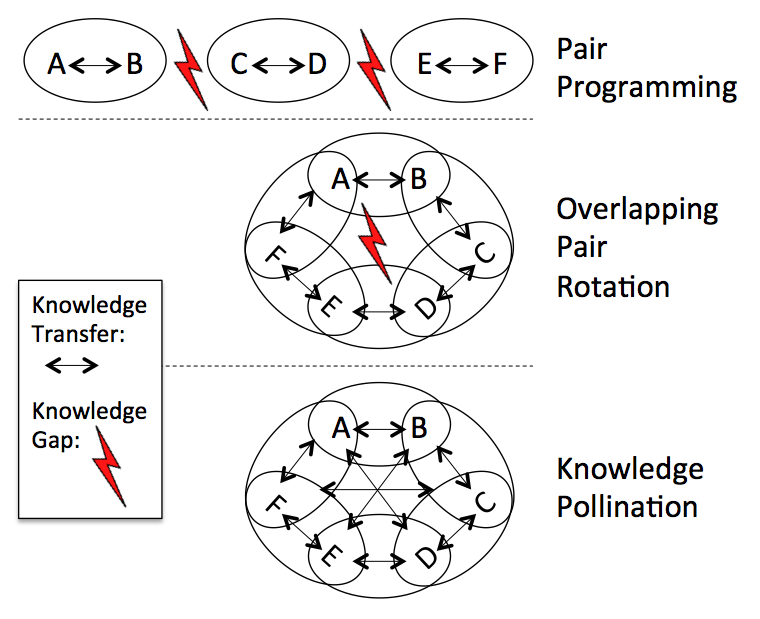
\includegraphics[width=\oneColumnWidth{}]{sustainable_software_development_images/KnowledgeSharingLevels.png}
\caption{Three Levels of Knowledge Sharing}
\label{KnowledgeSharing}
\end{figure}

\subsubsection{Continuous Pair Programming}
\textbf{Description:} Continuous Pair Programming is two developers collaborating to write software together as their normal mode of software development.

\textbf{Purpose:} When two developers work together, they are likely to bring more knowledge, and generate more diverse solutions compared to a solo developer. Additionally, there are many documented benefits of pair programming \cite {Williams2002}. When two developers work together, knowledge spreads from one developer to the next \cite{Zieris2016KnowledgeTransfer}, as illustrated in Figure 3. Overall, pairing reduces knowledge silos and can improve code quality.

\textbf{At Pivotal:} Pairing happens with two monitors, two keyboards, two mice, and one computer. Developers always work in pairs, unless exceptional circumstances arise. For instance, solo programming occurs when one developer is out of the office for part of the day (e.g. at home to let a plumber in, or at the doctor's office), out of the office the whole day (e.g. out sick), or involved in another business activity for a few hours (e.g. interviewing candidates, scoping a new project). When solo programming, developers take low-risk chores, refactorings, or stories. With any sizable project, there usually is something the team has been meaning to do that one person can safely do and report back to the team on its completion. 

\textbf{Anti-pattern:} Removing this practice results in solo programming where there is a clear owner for the code written. This would increase individual ownership and start creating knowledge silos. 

\textbf{Alternatives:} In solo programming, to remove silos, developers could take the stories for the part of the code they know least about. Assigning stories to developers who have the least understanding of the code could be a hard sell to management as it slows productivity down (at least initially). Bird's study \cite{BirdDontTouchMyCode} suggests that this approach would introduce more defects. 

\subsubsection{Overlapping Pair Rotation}
\textbf{Description:} Overlapping Pair Rotation happens when there is a rotation of the people working on a track of work: one developer rolls off and another developer rolls on. This results in knowledge continuity for a track of work, as illustrated in Figure 3. Typically, rotations happen in the morning as the evenings provide a natural interruption to the work. 

\textbf{Purpose:} The rotation of developers helps spread knowledge and promotes team code ownership. The goal is to prevent the situation where one or two developers understands how  part of the system works and must be on any story related to that part of the system. The entire team should be able to modify the code. Rotation helps prevent knowledge silos and individual code ownership from forming. 

\textbf{At Pivotal:} Whenever a knowledge silo begins to emerge, the team actively fights against it and tries to spread that knowledge around through pair rotation. Currently, there are three strategies in use. 

\textit{Optimizing for people rotation:} Most teams rotate based on who has paired with whom. Developers try to pair with the person they \quotes{least recently paired with} (basically a Least Recently Used strategy). Some teams use rotation techniques or tools to track this information.

As a downside, the strategy does not clearly articulate the purpose of knowledge silo removal and the need for knowledge transfer. As an example, developers who recently left a track of work might ask to be rotated back without realizing the potential cost to the team. This prevents an opportunity to spread the knowledge to the rest of the team. (On a four person team, this is not an issue).

\textit{Optimizing for personal preferences:} A few teams allow developers to pick with whom they will work or on which stories to work based on individual preferences. This has the same downsides as the previous strategy. 

\textit{Optimizing for context sharing:} A few teams are experimenting with rotating onto a track the person who has not been working on the track for the longest time. The goal each day is for the developer leaving the track next to empower the developer whom will remain on the track. Before any rotation, the remaining developer is asked, \quotes{Was enough context shared with you?} If the answer is no, then the first developer does not leave and the pair continues to work together for another day. This provides a feedback loop on how well the team is transferring knowledge. 

\textbf{Anti-pattern:} Removing this practice means that developers can work on the same part of the code base for extended periods of time, developing individual code ownership and knowledge silos. One participant described their experience at a previous company that follows Extreme Programming. Developers could be paired for more than a month working on only one part of the system. This lack of pair rotation led to deep knowledge silos. 

Ideally, developers work on the next, non-blocked story at the top of the backlog. When developers start skipping down the backlog, it can be an indication that they might not have enough context to work on any story. On Project Quattuor, a knowledge silo emerged around a complicated bug related to an obsolete technology that only a handful of people understood. Often developers would skip over stories and bugs related to that technology. At one point, the product manager reminded the team to keep \quotes{working from the top of backlog.}

Sometimes a developer wants to see a story through to completion over multiple days. Maybe he or she loves the technology or the feature. In these situations, the team needs to be careful about forming knowledge silos and creating a sense of personal ownership. If the team says \quotes{We need Marion on that story, only she really knows the Apple watch code base,} or \quotes{Shea knows the ins-and-outs of the legacy integration, we need him to work on this story,} then these are signs that knowledge silos have emerged. 

\textbf{Alternatives:} Team members that build a knowledge silo can share what they learned through a demo, code walk through, or a team huddle. This helps a team share knowledge, but is less effective than working directly with the code. 

\subsubsection{Knowledge Pollination}
\textbf{Description:} Knowledge Pollination refers to the set of activities contributing to knowledge sharing in an unstructured way. Examples include daily stand-up meetings, weekly retrospections, writing or sketching on whiteboards, overhearing a conversation, using the backlog to communicate current status about a story, calling out an update to the entire team, or simply reaching out to others to ask questions as needed. 

\textbf{Purpose:} Knowledge Pollination contributes to spreading knowledge among the team as illustrated in Figure 3.

\textbf{At Pivotal:} Daily standups create awareness of who is working on what. Teams can write down a \quotes{parking lot} of issues to discuss during daily standups. A pair may record the current status of a blocked story so that the next pair picking it up knows the situation. Osmotic communication helps when a developer overhears another pair discussing an issue and offers needed knowledge. Instead of thrashing, a pair interrupts another pair to gain the needed information. Thus, interruptions are encouraged as they make the entire team more efficient as knowledge pollinates across the team. 

Calling out an update to the entire team might be a simple as shouting \quotes{The build is broken, we are looking into it}, or this interchange: \quotes{We just checked in a presenter,} followed by \quotes{We just used your presenter. That's great collaboration.}

While working on a story, a pair may discover that they are missing some key context that prevents them from efficiently proceeding. If the issue is about the acceptance criteria for a story, they clarify with the product manager. If the issue is about the code base, the pair can ask the people who recently worked on that section of code, or ask the entire team. To determine whom to ask, the pair may remember who did what at stand-up, look through Pivotal Tracker to see who worked on a story, or check out source code version history (e.g. git annotate). Two-, four-, and six- person teams tend to have collective memory of who worked on which features from daily standup. 

These mechanisms help a team build awareness. Chong observed that \quotes{transmission of awareness information is a relatively effortless act in the XP environment} in her ethnographic study of an Extreme Programming team compared to a traditional team \cite{ChongNominum}.
 
\textbf{Anti-pattern:} An organization that provides little opportunity to share knowledge leads to wasted time as developers must acquire the knowledge through other means or end up reinventing the wheel.
\subsection{Caretaking the Code Practices}
\subsubsection{Test-Driven Development, Behavior-Driven Development}
\textbf{Description:} In Test-Driven Development (TDD) developers write unit tests before creating a design and writing code. In Behavior-Driven Development (BDD) developers implement acceptance tests before creating a design and writing code. Most lines of production code are tested before the production code is written. The software's design emerges from the tests and subsequent refactorings.

In Extreme Programming, Kent Beck describes his corresponding \quotes{Testing} practice as developers writing \quotes{automated unit tests} and implementing customer provided \quotes{functional tests} for story acceptance \cite{BeckExtremeProgramming2000}. Later, Kent Beck refines these ideas as \quotes{Test-first programming} \cite{BeckExtremeProgramming2004}. 

\textbf{Purpose:} This practice creates a safety net and empowers a pair to have the confidence to modify the code base. This enables any pair to pick up any story. Continuous Refactoring results in easier to modify tests.

\textbf{At Pivotal:} Developers use a combination of TDD and BDD. While each project is different, programmers tend to use BDD to describe interactions between the user and the system and TDD at a unit test level. Teams use a variety of TDD strategies including testing the responsibilities and interactions \cite{Goose} or contract testing using mocks as described by J. B. Rainsberger \cite{RainsbergerIntegrationTestsYouTube}. In Pivotal's ideal, the design emerges from the creation and exploration of the test cases. 

\textbf{Anti-pattern:} Removing this testing practice means that developers no longer have the confidence to change any part of the code as they may unknowingly end-up breaking something else. 

\textbf{Alternatives:} For a system without a test suite documenting the system specification, a possible remedy is creating knowledge silos where developers own particular parts of the system and understand the ramifications of changes. Creating strong code ownership is exactly the problem that sustainable software development is trying to solve.

Writing tests after the code is written could produce a safety net for refactoring, provided that tests correctly exercise the system. (A test that was never red might not be testing anything). We did not observe this behavior and future research is necessary to determine if any testing approach is sufficient for sustainable software development.

\subsubsection{Continuous Refactoring}
\textbf{Description:} Continuous Refactoring is the systematic improvement of the code base while feature work is being performed. When developers identify something wrong such as a code smell, they simply fix it. In this regard, developers are caretaking the code by continuously improving it. This practice results in an emergent software design, as well as empathy for the code as developers learn to \quotes{listen to the code.} 

%Continuous Refactoring is one way to prevent technical debt from accumulating. When a team employs continuous refactoring, the team refines a code base towards simple design, intention revealing code, and discoverable code. 

\textbf{Purpose:} Continuous Refactoring enables any pair to work on any part of the system. Taking the time to increase code discoverability, code readability, code modifiability, and code simplicity produces long-term benefits for the team. 

\textbf{At Pivotal:} Developers typically do some refactoring while implementing stories. Developers are encouraged to improve the code's design, make the code easier to understand, and increase the discoverability of a component based upon its responsibility. Usually, the team prefers \quotes{pre-factoring} where the developer does the complicated work to make the implementation of the current story as simple and easy as possible, as opposed to \quotes{post-factoring} where refactoring happens after the story is done, but before it is delivered. 

\textbf{Anti-pattern:} Removing this practice might produce hard to modify and messy code. Developers might not be able to easily work on any part of the code base. When refactoring is skipped, code might be simply bolted on to the existing design. Soon it becomes increasingly difficult to bolt more code on. A dilemma arises for the programmers working on the next story: do they continue bolting on more code, or do they perform the pretermitted refactorings? Removing this practice may also result in hard-to-change tests.

\textbf{Alternatives:} There are extreme situations where postponing refactoring for later becomes necessary. For instance, when the company might go out of business unless the company releases the next version. These moments should be considered carefully. The team risks taking on uncontrolled technical debt as \quotes{refactoring later} turns into \quotes{refactoring never.} 

\subsubsection{Live on Master}
\textbf{Description:} Live on master means that developers integrate their code several times a day, as quickly as possible. ExtremeProgramming.org calls this practice \quotes{Integrate Often.} \cite{WellsIntegrateOften} 

\textbf{Purpose:} For teams to continuously refactor and minimize the waste of merge conflicts, the entire team needs to be routinely merging their code onto master. If a pair communicates to the team that they are actively \quotes{refactoring} a component, they are asserting exclusive temporary ownership over the file to avoid merge conflicts. While this is a normal practice for a few hours, if it happens for multiple days, the team is losing collective ownership of that code. The team is not able to receive any of the benefits until the work is merged back to master. 

\textbf{At Pivotal:} In the ideal workflow, developers merge their code to master many times a day. If a pair has not merged to master by the afternoon, the pair typically starts examining why this is difficult and explores ways of incrementally making changes. Developers may use branches to save spikes. When rotating pairs, developers may use branches to move work-in-progress code between machines. 

\textbf{Anti-pattern:} Removing this practice means that code lives in branches for days or weeks. Integrations might be painful due to merge conflicts and developers might delay needed refactorings. If a developer has code only on their machine, then no one else on the team can use or modify that code. When code lives only on one machine for many days in a row, the machine acts as a \quotes{virtual branch.} Running a Continuous Integration box and having long running branches is an anti-pattern.
\section{Theory Evaluation}
\label{TheoryEvaluation}

In assessing a Grounded Theory research study, Charmaz identifies four criteria for evaluating the theory: credibility (\quotes{Is there sufficient data to merit claims?}), originality (\quotes{Do the categories offer new insights?}), resonance (\quotes{Does the theory make sense to participants?}), and usefulness (\quotes{Does the theory offer useful interpretations?}) \cite{StolGTinSE}. 

\textbf{Credibility:} The current data set is rich and lead to theory saturation. (Saturation means that the properties of the theory are complete and are not affected by new data). The data set comprises 21 intensive interviews conducted in four different offices, field notes from participant observation on Project Quattuor, and the primary researcher's involvement in four other projects as participant-observer.

\textbf{Originality:} The theory uniquely depicts the principles, policies, and practices enabling software development sustainability in an organization. Since the organization under study follows Extreme Programming, it is not surprising that many of the practices of Sustainable Software Development are defined in Extreme Programming. However, overlapping pair rotation and its supporting principles, policies, and practices are central and unique to the proposed theory.

\textbf{Resonance:} The theory has been presented to the participants. The theory made sense and reflects the way they work. 

\textbf{Usefulness:} The theory informs Pivotal engineers as to why Pivotal purposefully avoids knowledge silos, and how the theory's principles, policies, and practices work together to accomplish the team's goals. The theory explains why the principles, policies, and practices should be incorporated together without taylorization. A few managers use  the theory to help potential clients understand how Pivotal achieves the business goals of both the client and Pivotal.

\section{Threats to Validity}

\subsection{External Validity}

\textbf{Generalizability across situations:} Grounded theory does not support statistical generalization from a sample to a population. The results may not be applicable to other teams or other domains. There are four broad types of scientific generalization: 1) from data to descriptions, 2) from descriptions to concepts, 3) from concepts to theory, 4) from theory to description \cite{Lee2003generalizing}. Grounded theory research involves the first three kinds of generalization. Generalizing from a theory confirmed in one context to descriptions of a new context (the fourth kind of generalization) could be done by the researchers in the new context, on a case-by-case basis. However, we have not attempted to perform any type four generalizations at this time.

\subsection{Internal Validity}
\textbf{Researcher bias:} A risk of the participant-observer technique is that the researcher may lose perspective and become biased by being a member of the team. An outside observer might see something the researcher missed. We mitigated this risk by recording interviews and with a colleague reviewing the coding process.

\textbf{Prior knowledge bias:} With grounded theory, prior knowledge can aid the researcher in looking at interesting research questions or create difficulties by blinding the researcher about possible explanations \cite{GlaserIssues}. We mitigated this risk with a colleague reviewing the coding process. 
\section{Future Research}
We are interested in the tension between individual and team ownership, as well as the factors that foster and decrease the sense of ownership. Developers, interaction designers, and product managers all have different goals for their role. In future work, we plan to examine how the sense of ownership is driven by different factors for each role.

Some programmers naturally adapt to team code ownership, while others struggle with the transition. In future research we will follow new Pivotal engineers and examine their journey in transitioning from individual code ownership to team code ownership. Perhaps there are 
specific practices that Pivotal or the development team could employ to ease the transition. We will also investigate the optimal team size for team code ownership. 

\section{Conclusions}
This paper introduces a descriptive theory of \quotes{Sustainable Software Development} as a solution to the challenge of software development sustainability for an ever changing workforce. The theory emerged from a Constructivist Grounded Theory research study. By collecting data from 21 intensive interviews conducted in four different Pivotal offices, field notes from participant-observation on the Project Quattuor, and the primary researcher's involvement in four other Pivotal projects as participant-observer, the study investigates the research question \quotes{How do the observed teams develop software effectively while overcoming team disruption?}

The emergent theory is characterized by a collection of synergistic principles, policies, and practices encouraging a positive attitude towards team disruption, knowledge sharing and continuity, as well as caring about code quality. The theory refines and extends the understanding of Extreme Programming by adding a few principles, policies, and practices (like the unique Overlapping Pair Rotation practice) and aligning these principles, policies, and practices towards the business goal of sustainability.

Conventional wisdom says that team disruptions should be avoided, and that extensive documentation is needed to prevent knowledge loss during team churn. Unfortunately, documentation often quickly becomes out-of-date and unreliable, making this approach suboptimal. The theory positions team code ownership with overlapping pair rotation and knowledge pollination as an alternative and potentially more effective strategy to mitigate against knowledge loss.

The primary benefits to the software developer are the ability to understand the entire system, to work on every story, an increase in teaching opportunities to share one's expertise, and in-depth opportunities to learn the subtle parts of the utilized technologies. 

The primary benefit to the employer is business agility. The engineering team continues to deliver software week after week, month after month, while surviving cataclysmic events. Things do not fall apart when the superstar developer leaves because features or components are not critically tied to a particular individual. Critical feature work can be parallelized since anyone can work on the feature, as opposed to an individual code owner.  The team leverages the whole team's talents. Sustainable Software Development is suited for companies that must routinely deliver value to their users, customers, or stakeholders. 

\section{Acknowledgement}

Thank you to Rob Mee, David Goudreau, Ryan Richard, and Zach Larson for making this research possible. Thank you to Karina Sils for creating Figure \ref{PlannedDeveloperStaffing} and Figure \ref{DeveloperStaffing} using Sketch.
